\part{Teoria della computabilità}
\chapter{La tesi di Church-Turing}
\section{Macchine di Turing}
Introduciamo ora un modello molto più potente, proposto inizialmente da Alan Turing nel 1936, chiamato macchina di Turing. Simile ad un automa finito, ma con una memoria illimitata e senza restrizioni, una macchina di Turing è un modello molto più preciso di un computer. Una macchina di Turing può fare tutto ciò che può fare un computer reale. 

Una macchina di Turing utilizza un nastro infinito come propria memoria illimitata. Ha una testina che è in grado di leggere e scrivere simboli ed è libera di muoversi lungo il nastro. Inizialmente il nastro contiene solo la stringa di input e tutto il resto è vuoto. Se la macchina deve memorizzare un'informazione, la può scrivere sul nastro. Per leggere l'informazione che ha scritto, la macchina può spostare la testina su di essa. La macchina continua a computare finché non decide di produrre un output. Gli output "accetta" e "rifiuta" sono ottenuti occupando appositi stati di accettazione e di rifiuto. Se non raggiunge uno stato di accettazione o di rifiuto, la macchina andrà avanti per sempre, senza mai fermarsi.

Quindi una macchina di Turing:
\begin{enumerate}
    \item può sia scrivere che leggere sul nastro;
    \item ha una testina di lettura-scrittura può muoversi sia verso sinistra che verso destra;
    \item ha un nastro infinito;
    \item ha degli stati speciali di accettazione e rifiuto che hanno effetto immediato.
\end{enumerate}

\begin{Example}{Macchina di Turing}{}
\textit{Introduciamo una macchina di Turing $M_{1}$ per testare l'appartenenza al linguaggio $B=\{ w\#w |w \in\{ 0,1\}^*\}$.}

Vogliamo che $M_{1}$ accetti se l'input è un elemento di $B$ e che rifiuti altrimenti, cioè se l'input comprende due stringhe identiche separate da un simbolo \#. La strategia ovvia è quella di muovervi a zig-zag in maniera simmetrica attorno al simbolo \# e stabilire se gli elementi nelle posizioni di ugual indice su i due lati corrispondono. Contrassegnate poi il nastro per tenere traccia degli elementi che corrispondono. 

Progettiamo $M_{1}$ in modo da lavorare in questo modo. Esegue più passaggi sulla stringa in input con la testina di lettura-scrittura. Ad ogni passaggio verifica la corrispondenza di un carattere ad ogni lato del simbolo \#. Per tenere traccia dei simboli già controllati, $M_{1}$ barra ogni simbolo già esaminato. Se ha barrato tutti i simboli, significa che tutti i simboli corrispondevano ed $M_{1}$ va in uno stato di accettazione. Se si accorge di una mancata corrispondenza, $M_1$ entra in uno stato di rifiuto.
\end{Example}

\subsection{Definizione formale di macchina di Turing}
Il cuore della definizione di una macchina di Turing è la funzione di transizione, perché essa ci dice come la macchina effettua un passo. Per una macchina di Turing, $\delta$ prende la forma $Q\times\Gamma\to Q\times \Gamma\times\{L, R\}$. Cioè, quando la macchina occupa un certo stato $q$ e la testina punta alla casella del nastro contenente un simbolo $a$, e se $\delta(q, a) = (r, b, L)$ la macchina scrive il simbolo $b$ al posto di $a$, e passa nello stato $r$. La terza componente è $L$ oppure $R$ ed indica se la testina si sposta verso sinistra o verso destra dopo la scrittura. In questo caso la $L$ indica una mossa a sinistra.

\begin{Definition}{Macchina di Turing}{}
Una macchina di Turing è una 7-tupla, $(Q, \Sigma, \Gamma, \delta, q_0, q_{accept}, q_{reject})$, dove $Q, \Sigma, \Gamma$ sono tutti insiemi finiti e
\begin{enumerate}
    \item $Q$ è l'insieme degli stati,
    \item $\Sigma$ è l'alfabeto di input non contenente il simbolo blank $\sqcup$,
    \item $\Gamma$ è l'alfabeto del nastro, con $\sqcup \in\Gamma$ e $\Sigma\subseteq\Gamma$,
    \item $\delta: Q\times\Gamma\to Q\times\Gamma\times\{L, R\}$ è la funzione di transizione,
    \item $q_{0} \in Q$ è lo stato iniziale,
    \item $q_{accept}\in Q$ è lo stato di accettazione e
    \item $q_{reject}\in Q$ è lo stato di rifiuto, con $q_{reject}\neq q_{accept}$.
\end{enumerate}
\end{Definition}

Una macchina di Turing $M=( Q, \Sigma, \Gamma, \delta, q_{0}, q_{accept}, q_{reject})$ computa nel seguente modo. Inizialmente $M$ riceve il suo input $w= w_{1}w_{2}...w_n\in\Sigma^*$ sulle $n$ celle più a sinistra del nastro, mentre il resto del nastro è vuoto (cioè, contiene tutti simboli blank). La testina parte dalla posizione più a sinistra del nastro. Si noti che $\Sigma$ non contiene il simbolo blank, in tal modo il primo simbolo blank che compare sul nastro segna la fine dell'input. Quando $M$ inizia la computazione, questa procede secondo le regole descritte dalla funzione di transizione. La computazione prosegue fin quando la macchina raggiunge lo stato di accettazione oppure di rifiuto, a tal punto si ferma. Se nessuno dei due stati viene raggiunto, $M$ va avanti per sempre. 

Durante la computazione di una macchina di Turing, si verificano cambiamenti dello stato corrente, del contenuto corrente del nastro, e della posizione corrente della testina. Un'impostazione di questi tre elementi è chiamata una configurazione della macchina di Turing. Le configurazioni sono spesso rappresentate in modo speciale. Per uno stato $q$ e due stringhe $u$ e $v$ sull'alfabeto $\Gamma$ del nastro, scriviamo $uqv$ per indicare la configurazione, dove lo stato corrente è $q$, il contenuto corrente del nastro è $uv$ e la posizione attuale della testina è il primo simbolo di $v$. Dopo l'ultimo simbolo di $v$, il nastro contiene solo simboli blank. 

Si dice che la configurazione $C_{1}$ produce la configurazione $C_{2}$ se la macchina di Turing può passare da $C_{1}$ a $C_{2}$ in un unico passo. Definiamo formalmente questa nozione nel seguente modo. Supponiamo di avere $a$, $b$ e $c$ in $\Gamma$, così come $u$ e $v$ in $\Gamma^*$ e gli stati $q_{i}$ e $q_j$. In tal caso $uaq_{i}bu$ e $uq_{j}acv$ sono due configurazioni. Diciamo che 
\begin{equation*}
    uaq_ibv \textit{ produce } uq_jacv
\end{equation*}
se nella funzione di transizione $\delta(q_{i}, b) = (q_{j}, c, L)$. Questo nel caso in cui la macchina di Turing effettua verso sinistra. Per uno spostamento a destra, diciamo che
\begin{equation}
    uaq_ibv \textit{ produce }uacq_jv
\end{equation}
Una macchina di Turing $M$ accetta l'input $w$ se esiste una sequenza di configurazioni $C_{1}, C_{2} ,...,C_k$ tale che
\begin{enumerate}
    \item $C_{1}$ è la configurazione iniziale di $M$ su input $w$,
    \item ogni $C_{i}$ produce $C_{i+1}$ e
    \item $C_{k}$ è una configurazione di accettazione.
\end{enumerate}
L'insieme di stringhe che $M$ accetta rappresenta il linguaggio di $M$, o il linguaggio riconosciuto da $M$, denotato con $L(M)$.

\begin{Definition}{Linguaggio Turing-riconoscibile}{}
Un linguaggio si dice Turing-riconoscibile se esiste una macchina di Turing che lo riconosce.
\end{Definition}

Quando attiviamo una macchina di Turing su un input, tre risultati sono possibili. La macchina può accettare, rifiutare, oppure andare in loop (ciclare). Per loop si intende semplicemente che la macchina non si ferma. Un ciclo, in quanto tale, comporta un qualche comportamento semplice o complesso che non porta ad uno stato di arresto. Una macchina che non va in loop è detta decisore perché prende in ogni caso una decisione, sia essa di accettare o di rifiutare. 

\begin{Definition}{Linguaggio Turing-decidibile}{}
Un linguaggio si dice Turing-decidibile o semplicemente decidibile se esiste una macchina di Turing che lo decide.    
\end{Definition}

\begin{Example}{Linguaggio Turing-riconoscibile}{}
La seguente macchina di Turing riconosce il linguaggio $L = \{01^n0| n\geq0\}$.

\begin{minipage}{\textwidth}
    \centering
    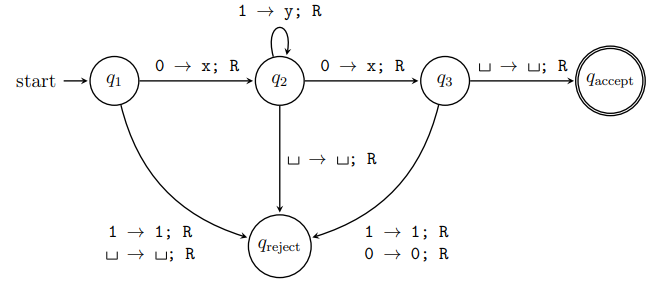
\includegraphics[width=0.7\textwidth]{images/es-linguaggio-turing-riconoscibile.PNG}
    %\captionof{figure}{}
\end{minipage}

Infatti, durante la lettura della stringa \texttt{01110}, la macchina assume le seguenti
configurazioni:
\begin{align*}
&q_1\text{ }0\text{ }1\text{ }1\text{ }1\text{ }0\\
&x\text{ }q_2\text{ }1\text{ }1\text{ }1\text{ }0\\
&x\text{ }y\text{ }q_2\text{ }1\text{ }1\text{ }0\\
&x\text{ }y\text{ }y\text{ }q_2\text{ }1\text{ }0\\
&x\text{ }y\text{ }y\text{ }y\text{ }q_2\text{ }0\\
&x\text{ }y\text{ }y\text{ }y\text{ }x\text{ }q_3\text{ }\sqcup\\
&x\text{ }y\text{ }y\text{ }y\text{ }x\text{ }\sqcup\text{ }q_{accept}\text{ }\sqcup
\end{align*}
\end{Example}

\begin{Example}{Linguaggio Turing-riconoscibile}{}
La seguente macchina di Turing riconosce il linguaggio $L = \{0^n1^n| n\geq0\}$.

\begin{minipage}{\textwidth}
    \centering
    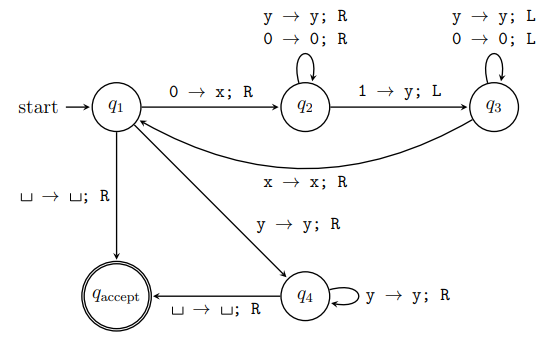
\includegraphics[width=0.6\textwidth]{images/es-linguaggio-turing-riconoscibile2.PNG}
    %\captionof{figure}{}
\end{minipage}

Infatti, durante la lettura della stringa \texttt{000111}, la macchina assume le seguenti configurazioni:
\begin{center}
\begin{tabular}{l l l l}
$q_1\text{ }0\text{ }0\text{ }0\text{ }1\text{ }1\text{ }1$&$x\text{ }q_1\text{ }x\text{ }0\text{ }y\text{ }1\text{ }1$&$x\text{ }x\text{ }q_1\text{ }0\text{ }y\text{ }y\text{ }1$&\\
$x\text{ }q_2\text{ }0\text{ }0\text{ }1\text{ }1\text{ }1$&$x\text{ }x\text{ }q_2\text{ }0\text{ }y\text{ }1\text{ }1$&$x\text{ }x\text{ }x\text{ }q_2\text{ }y\text{ }y\text{ }1$&$x\text{ }x\text{ }x\text{ }q_3\text{ }y\text{ }y\text{ }y$\\
$x\text{ }0\text{ }q_2\text{ }0\text{ }1\text{ }1\text{ }1$&$x\text{ }x\text{ }0\text{ }q_2\text{ }y\text{ }1\text{ }1$&$x\text{ }x\text{ }x\text{ }y\text{ }q_2\text{ }y\text{ }1$&$x\text{ }x\text{ }x\text{ }y\text{ }q_4\text{ }y\text{ }y$\\
$x\text{ }0\text{ }0\text{ }q_2\text{ }1\text{ }1\text{ }1$&$x\text{ }x\text{ }0\text{ }y\text{ }q_2\text{ }1\text{ }1$&$x\text{ }x\text{ }x\text{ }y\text{ }y\text{ }q_2\text{ }1$&$x\text{ }x\text{ }x\text{ }y\text{ }y\text{ }q_4\text{ }y$\\
$x\text{ }0\text{ }q_3\text{ }0\text{ }y\text{ }1\text{ }1$&$x\text{ }x\text{ }0\text{ }q_3\text{ }y\text{ }y\text{ }1$&$x\text{ }x\text{ }x\text{ }y\text{ }q_3\text{ }y\text{ }y$&$x\text{ }x\text{ }x\text{ }y\text{ }y\text{ }y\text{ }q_4\text{ }\sqcup$\\
$x\text{ }q_3\text{ }0\text{ }0\text{ }y\text{ }1\text{ }1$&$x\text{ }x\text{ }q_3\text{ }0\text{ }y\text{ }y\text{ }1$&$x\text{ }x\text{ }x\text{ }q_3\text{ }y\text{ }y\text{ }y$&$x\text{ }x\text{ }x\text{ }y\text{ }y\text{ }y\text{ }\sqcup\text{ }q_{accept}\text{ }\sqcup$\\
$q_3\text{ }x\text{ }0\text{ }0\text{ }y\text{ }1\text{ }1$&$x\text{ }q_3\text{ }x\text{ }0\text{ }y\text{ }y\text{ }1$&$x\text{ }x\text{ }q_3\text{ }x\text{ }y\text{ }y\text{ }y$&
\end{tabular}
\end{center}
\end{Example}

\section{Varianti di macchine di turing}
Esistono molte definizioni alternative di macchine di Turing, comprese le versioni multinastro o non deterministiche. Sono dette varianti del modello macchina di Turing. Il modello originale e le sue ragionevoli varianti hanno tutti lo stesso potere computazionale riconoscono la stessa classe di linguaggi. 

Per illustrare la robustezza del modello di macchina di Turing cerchiamo di variare il tipo di funzione di transizione consentito. Nella nostra definizione, la funzione di transizione forza la testina a spostarsi verso sinistra o destra ad ogni passo; la testina non può semplicemente restare ferma. Supponiamo di aver permesso alla macchina di Turing la capacità di restare ferma. La funzione di transizione avrebbe allora la forma $\delta: Q\times \Gamma\times \{L,R,S\}$. Siamo in grado di convertire qualsiasi TM con la possibilità di "restar ferma" in una che non ha tale capacità. Lo facciamo sostituendo ogni transizione "resta ferma" con due transizioni, una che sposta la testina a destra e una che la riporta a sinistra. Questo piccolo esempio contiene la chiave per mostrare l'equivalenza di varianti di TM. Per dimostrare che due modelli sono equivalenti abbiamo semplicemente bisogno di dimostrare che ognuno dei due può simulare l'altro.

\subsection{Macchina di Turing multinastro}
Una macchina di Turing multinastro è come una normale macchina di Turing con vari nastri. Ogni nastro ha la sua testina per la lettura e la scrittura. Inizialmente l'input si trova sul nastro 1, mentre gli altri nastri sono vuoti. La funzione di transizione viene modificata per consentire la lettura, la scrittura e lo spostamento della testina contemporaneamente su alcuni o tutti i nastri. Formalmente,

\begin{equation*}
    \delta: Q\times\Gamma^k\rightarrow Q\times \Gamma^k\times \{L, R, S\}^k
\end{equation*}
dove $k$ è il numero di nastri. L'espressione
\begin{equation*}
    \delta( q_{i}, a_{1} ,...,a_k)=(q_j ,b_1 ,...,b_k ,L,R,...,L)
\end{equation*}
significa che, se la macchina si trova nello stato $q_{i}$ e le testine da 1 a $k$ leggono i simboli da $a_{1}$ ad $a_{k}$, la macchina va nello stato $q_{j}$ scrive i simboli da $b_{1}$ a $b_{k}$ e muove ogni testina a sinistra o a destra, o la fa restare ferma, come specificato.

\begin{Thm}{Turing multinastro è equivalente a Turing singolo nastro}{}\label{thm:Tmulti-TM}
\textit{Per ogni macchina di Turing multinastro esiste una macchina di Turing a nastro singolo equivalente.}

\begin{demonstration}
Mostriamo come convertire una macchina di Turing multinastro $M$ in una TM $S$ equivalente a nastro singolo. L'idea chiave è quella di mostrare come simulare $M$ con $S$. Supponiamo che $M$ abbia $k$ nastri. Allora $S$ simula l'effetto di $k$ nastri memorizzando le loro informazioni sul suo singolo nastro. Essa utilizza il nuovo simbolo $\#$ come delimitatore per separare i contenuti dei diversi nastri. Oltre al contenuto dei nastri, $S$ deve tenere traccia delle posizioni delle testine. Lo fa scrivendo un simbolo con un punto sopra per contrassegnare la posizione in cui si troverebbe la testina di quel nastro. Pensate a questi come nastri e testine "virtuali". Come in precedenza, i simboli del nastro "puntati" sono semplicemente simboli nuovi che sono stati aggiunti all'alfabeto del nastro. 

$S= \textit{"Su input }w = w_1... w_n$:
\begin{enumerate}
    \item Inizialmente $S$ mette il suo nastro nel formato che rappresenta tutti i $k$ nastri di $M$. Il nastro formattato contiene
    \begin{equation*}
        \# \overset{\bullet}{w_1}w_2...w_n\# \overset{\bullet}{\sqcup}\#\overset{\bullet}{\sqcup}\#...\#
    \end{equation*}
    \item Per simulare una singola mossa, $S$ scansiona il suo nastro dal primo $\#$, che segna l'estremità sinistra, al $(k+1)$mo $\#$, che segna l'estremità di destra, per determinare i simboli puntati dalle testine virtuali. Successivamente $S$ fa un secondo passaggio per aggiornare i nastri in accordo alla funzione di transizione di $M$.
    \item Se in qualsiasi momento $S$ sposta una delle testine virtuali a destra su un $\#$, questa azione significa che $M$ ha spostato la testina corrispondente sulla parte di nastro vuota non letta in precedenza. Quindi $S$ scrive un simbolo blank in questa cella del nastro e sposta il contenuto del nastro, da questa cella fino al simbolo $\#$ più a destra, di una unità a destra. Poi prosegue la simulazione come prima."
\end{enumerate}    
\end{demonstration}
\end{Thm}

\begin{Corollario}{Linguaggio Turing-riconoscibile e Turing multinastro}{}
\textit{Un linguaggio è Turing-riconoscibile se e solo se qualche macchina di Turing multinastro lo riconosce.}

\begin{demonstration}
Un linguaggio Turing-riconoscibile è riconosciuto da una macchina di Turing ordinaria (ad un solo nastro), che è un caso particolare di una macchina di Turing multinastro. Questo prova un verso di questo corollario. L'altro verso segue dal Teorema \ref{thm:Tmulti-TM}.
\end{demonstration}
\end{Corollario}

\subsection{Macchina di Turing non deterministica}
In una macchina di Turing non deterministica, in qualsiasi punto della computazione, la macchina può procedere effettuando varie scelte. La funzione di transizione di una macchina di Turing non deterministica è della forma
\begin{equation*}
    \delta: Q\times\Gamma\rightarrow\mathcal{P}(Q\times\Gamma\times\{L,R\})
\end{equation*}
La computazione di una macchina di Turing non deterministica è un albero i cui rami corrispondono alle diverse scelte possibili previste per la macchina. Se qualche ramo della computazione porta allo stato di accettazione, allora la macchina accetta l'input. Ora mostriamo che il non determinismo non influisce sulla potenza di calcolo del modello macchina di Turing.

\begin{Thm}{Turing non deterministica è equivalente a Turing deterministica}{}
\textit{Per ogni macchina di Turing non deterministica esiste una macchina di Turing deterministica equivalente.}

\begin{osservation}
Possiamo simulare qualsiasi TM non deterministica $N$ con una TM deterministica $D$. L'idea di base della simulazione consiste nel provare tutte le possibili scelte che può fare $N$ durante la sua computazione non deterministica. Se $D$ trova lo stato di accettazione su uno qualsiasi di questi rami, allora $D$ accetta. Altrimenti, la simulazione di $D$ non terminerà. Guardiamo alla computazione di $N$ su un input $w$ come ad un albero. Ogni ramo dell'albero rappresenta una scelta non deterministica. Ogni nodo dell'albero è una configurazione di $N$. La radice dell'albero è la configurazione iniziale. La TM $D$ esplora questo albero alla ricerca di una configurazione di accettazione. Eseguire accuratamente questa ricerca è cruciale perché con una ricerca in profondità $D$ potrebbe non visitare l'intero albero, entrando in un loop. Quindi progettiamo $D$ in modo da esplorare l'albero utilizzando, invece una visita in ampiezza (breadth-first search). Questa strategia esplora tutti i cammini che terminano alla stessa profondità prima di andare a esplorare ogni cammino che termina alla profondità successiva. Questo metodo garantisce che $D$ visita ogni nodo dell'albero finché non incontra una configurazione di accettazione.
\end{osservation}

\begin{demonstration}
La TM $D$ deterministica che simula ha tre nastri. La macchina $D$ utilizza i suoi tre nastri in maniera particolare. Il nastro 1 contiene sempre la stringa di input e non viene mai modificato. Il nastro 2 mantiene una copia del nastro di $N$ corrispondente a qualche diramazione della sua computazione non deterministica. Il nastro 3 tiene traccia della posizione di $D$ nell'albero delle computazioni di $N$.

% Consideriamo in primo luogo la rappresentazione dei dati sul nastro 3. Ogni nodo dell'albero può avere al massimo $b$ figli, dove $b$ è la dimensione del più grande insieme di scelte possibili date dalla funzione di transizione di $N$. Ad ogni nodo della struttura assegniamo un indirizzo che è una stringa sull'alfabeto $\Gamma_b=\{1,2,....b\}$. Assegniamo l'indirizzo 231 al nodo a cui si arriva partendo dalla radice, spostandosi al suo secondo figlio, spostandosi ancora da tale nodo al suo terzo figlio ed infine spostandosi al primo figlio di quest'ultimo nodo. Ogni simbolo della stringa ci dice quale deve essere la scelta successiva, durante la simulazione di un passo in una ramificazione di una computazione non deterministica di $N$. A volte un simbolo può non corrispondere ad una scelta se sono disponibili troppe poche scelte per una configurazione. In tal caso l'indirizzo non è valido e non corrisponde ad alcun nodo. Il nastro 3 contiene una stringa su $\Gamma_b$. Essa rappresenta la ramificazione della computazione di $N$ dalla radice al nodo indirizzato da tale stringa, a meno che l'indirizzo sia non valido. La stringa vuota è l'indirizzo della radice dell'albero. Siamo ora pronti a descrivere $D$.

\begin{enumerate}
    \item Inizialmente il nastro 1 contiene l'input $w$ e i nastri 2 e 3 sono vuoti.
    \item Copia il nastro 1 sul nastro 2 ed inizializza la stringa sul nastro 3 a $\epsilon$.
    \item Utilizza il nastro 2 per simulare $N$ con input $w$ su una ramificazione della sua computazione non deterministica. Prima di ogni passo di $N$, consulta il simbolo successivo sul nastro 3 per determinare quale scelta fare tra quelle consentite dalla funzione di transizione di $n$. Se non rimangono più simboli sul nastro 3 o se questa scelta non deterministica non è valida, interrompe questo cammino andando alla fase 4. Va alla fase 4 anche quando si verifica una configurazione di rifiuto. Se incontra una configurazione di accettazione, allora accetta l'input.
    \item Sostituisce la stringa sul nastro 3 con la stringa successiva rispetto all'ordine sulle stringhe. Simula la ramificazione successiva della computazione di $N$ andando al passo 2.
\end{enumerate}
\end{demonstration}
\end{Thm}

\subsection{Enumeratori}
Definito in modo informale, un enumeratore è una macchina di Turing con una stampante collegata. La macchina di Turing può utilizzare tale stampante come dispositivo di output per stampare stringhe. Ogni volta che la macchina di Turing vuole aggiungere una stringa alla lista, invia la stringa alla stampante.
Un enumeratore $E$ inizia con un nastro di input vuoto. Se l'enumeratore non si ferma, esso può stampare un elenco infinito di stringhe. Inoltre, $E$ potrebbe generare le stringhe del linguaggio in qualsiasi ordine, eventualmente anche con ripetizioni.

\begin{Thm}{Linguaggio Turing-riconoscibile $\iff\exists$ un enumeratore}{}
\textit{Un linguaggio è Turing-riconoscibile se e solo se esiste un enumeratore che lo enumera.}

\begin{demonstration}
Come prima cosa, dimostriamo che se abbiamo un enumeratore $E$ che enumera un linguaggio $A$, allora esiste una TM $M$ che riconosce $A$. La TM $M$ funziona come segue.

$M=\textit{"Su input }w$:
\begin{enumerate}
    \item Esegue $E$. Ogni volta che $E$ genera una stringa, la confronta con $w$.
    \item Se $w$ appare nell'output di $E$, accetta."
\end{enumerate}

Chiaramente, $M$ accetta quelle stringhe che compaiono sulla lista di $E$". Ora occupiamoci dell'altra direzione. Se la TM $M$ riconosce un linguaggio $A$, possiamo costruire il seguente enumeratore $E$ per $A$. Sia $s_1, s_2, s_3,...$ una lista di tutte possibili stringhe in $\Sigma^*$.

$E=\textit{"Ignora l'input}$.
\begin{enumerate}
    \item Ripete i seguenti passi per $i = 1,2,3,...$
    \item Esegue $M$ per $i$ passi su ogni input, $s_1, s_2,..., s_i$.
    \item Se una qualche computazione accetta, stampa la corrispondente $s_j$."
\end{enumerate}

Se $M$ accetta una particolare stringa $s$, alla fine $s$ apparirà nella lista generata da $E$. In realtà, essa apparirà nella lista un numero infinito di volte, perché $M$ ritorna all'inizio su ogni stringa per ogni ripetizione del passo 1. Questa procedura fa sì che $M$ lavori in parallelo su tutte le possibili stringhe di input.
\end{demonstration}
\end{Thm}